%!TEX root = ../../Heun_Dale_Haney_A_dynamic_approach_to_input_output_modeling.tex
%%%%%%%%%%%%%%%%%%%%% chapter.tex %%%%%%%%%%%%%%%%%%%%%%%%%%%%%%%%%
%
% sample chapter
%
% Use this file as a template for your own input.
%
%%%%%%%%%%%%%%%%%%%%%%%% Springer-Verlag %%%%%%%%%%%%%%%%%%%%%%%%%%
%\motto{Use the template \emph{chapter.tex} to style the various elements of your chapter content.}
\motto{A motto.~\emph{\cite[p.~26]{Berry1998}}

\hfill---\emph{Wendell Berry}}


%%%%%%%%%%%%%%%%%%%%%%%%%%%%%%%%%%
%%%%%%%%%% Introduction %%%%%%%%%%
%%%%%%%%%%%%%%%%%%%%%%%%%%%%%%%%%%
\chapter{Accounting for the Wealth of Nations}
% Always give a unique label
\label{chap:acct_for_won}
% use \chaptermark{}
% to alter or adjust the chapter heading in the running head
\chaptermark{Wealth of Nations}
%%%%%%%%%%%%%%%%%%%%%%%%%%%%%%%%%%
%%%%%%%%%%%%%%%%%%%%%%%%%%%%%%%%%%
%%%%%%%%%%%%%%%%%%%%%%%%%%%%%%%%%%


%% \abstract{Each chapter should be preceded by an abstract (10--15 lines long) that summarizes the content. The abstract will appear \textit{online} at \url{www.SpringerLink.com} and be available with unrestricted access. This allows unregistered users to read the abstract as a teaser for the complete chapter. As a general rule the abstracts will not appear in the printed version of your book unless it is the style of your particular book or that of the series to which your book belongs.\newline\indent
%% Please use the 'starred' version of the new Springer \texttt{abstract} command for typesetting the text of the online abstracts (cf. source file of this chapter template \texttt{abstract}) and include them with the source files of your manuscript. Use the plain \texttt{abstract} command if the abstract is also to appear in the printed version of the book.}

%% Use the template \emph{chapter.tex} together with the Springer document class SVMono (monograph-type books) or SVMult (edited books) to style the various elements of your chapter content in the Springer layout.

\abstract*{**** Write the abstract. ****
Abstract.}




%%%%%%%%%% Intro summary %%%%%%%%%%
\section{[BRH] Summary of introduction}
\label{sec:intro_summary}
%%%%%%%%%%

In Chapter~\ref{chap:acct_for_won}.



%%%%%%%%%% Incomplete accounting %%%%%%%%%%
\section{[BRH] Incomplete national accounting}
\label{sec:incomplete_accounting}
%%%%%%%%%%

In Chapter~\ref{chap:acct_for_won}.



Why is society doing the accounting incorrectly? 
Because we do not have correct assumptions about the way the economy works. 
Why are our assumptions incorrect? 

%%%%%%%%%% Metaphors and Models %%%%%%%%%%
\section{Metaphors and models}
\label{sec:metaphors_and_models}
%%%%%%%%%%

As discussed in Section~\ref{sec:incomplete_accounting}, 
national accounting is incomplete, and
an objective for this book is to provide rigorous theoretical grounding for 
a better national accounting framework.
But, before moving ahead with developing that framework,
it is useful to consider how society has come to this point.
How is it that we don't routinely and comprehensively account for
important material and energy flows into, within, and out of the economy
in systems of national accounts?

The classical economists certainly appreciated the dependence of
economic activity on bio-physical processes.\cite{Hall2011, Cleveland1987, Dale2012}
However, somewhere between William Stanley Jevons' 1865
assessment that
``the very existence of Britain, as a great nation''~\cite[IV.3]{Jevons1865}
was tied to a continued supply of low-cost coal 
and Julian Simon's 1998 statement that
``natural resources are not finite in any economic sense,''~\cite[p.~54]{Simon1998} %chktex 38
the importance of the biosphere was lost.
In the following sections, we argue that
a contributing reason for incomplete national accounting
is that we have the wrong metaphor for the economy,
and we provide a suggestion for a better metaphor.


%+++++++++ The clockwork metaphor ++++++++++
\subsection{The clockwork metaphor}
\label{sec:clockwork_metaphor}
%+++++++++

Most economics textbooks today depict the economy 
as in Figure~\ref{fig:perp_motion_1}.
Goods and services flow from the production sector
to the household sector~(consumption)
in exchange for payments.
The factors of production (labor and capital)
flow from the household sector to the
production sector in exchange for wages and rents (income).
Attention is primarily focused on the circular flow
of money~(dashed line).

\begin{figure}[!ht]
\centering\
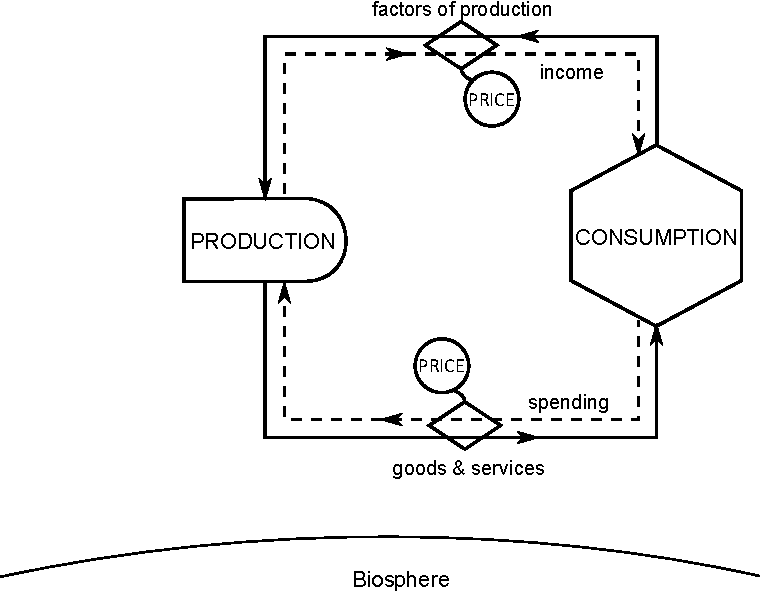
\includegraphics[width=\linewidth]{Part_0/Chapter_Introduction/images/Perpetual_motion_1.pdf}
\caption[The traditional model]{In the traditional model, the economy 
is represented as a circular flow of goods and services between two sectors. 
Producers manufacture goods and services 
by taking in labor and capital. 
Consumers exchange labor for wages 
which are used to purchase 
the goods and services of the producers.}
\label{fig:perp_motion_1}
\end{figure}

This traditional model of the economy~(Figure~\ref{fig:perp_motion_1}) 
is unashamedly mechanistic.
General equilibrium models of the economy
~\cite{Walras1892, Walras1993}
were borrowed directly from classical physics' models of 
mechanical equilibrium which, in turn, arose from the 
``clockwork universe'' metaphor.\cite{Ingrao1990}
The clockwork metaphor is a simplification 
that helps us make sense of the world around us.
Like all metaphors, it informs our thinking about the real world,
but, consequently,
it also constrains our ability to frame reality.
Erroneously, we mistake the model-metaphor for reality, and
we interact with reality in the same manner 
as we interact with the abstract objects of our
models.\footnote{This fallacious process is known as
	\emph{reification}; the making (\emph{facere}, Latin) real of
	something (\emph{res}, Latin) that is merely an idea.
	Alfred Whitehead refers to this as
	\emph{the fallacy of misplaced concreteness}.\cite{Whitehead2011}
	}
Classical physics told us the universe was
\emph{like} clockwork, 
so we began to interact with the universe
as if it \emph{really were} clockwork.
It then became easy to collect economic data that confirmed the clockwork model,
because the model told us which data to collect.

The clockwork metaphor and the traditional model of the economy
preclude any sort of connection 
between the economy and the biosphere.
Thus, only the internal dynamics of the economy are important. 
They tell us that natural resources are unimportant, 
effectively assuming that the biosphere will always provide.
If a particular resource becomes scarce, 
substitution to a different, more-readily-available resource will be made.
Wastes are quantitatively unimportant, 
effectively assuming that the biosphere has infinite assimilative capacity.
Economic forces (through prices and the market mechanism) 
are thought to effectively guide any necessary transition
within the economy.
With the clockwork metaphor, physical constraints 
imposed by the biosphere 
on allocation of resources, distribution of outputs, and 
scale of an economy 
are outside the scope of neoclassical economic discussion.\cite{Daly1995}
In short, the clockwork metaphor and the traditional model of the economy 
tell us that the clockwork-economy can and will carry on.

Because Figure~\ref{fig:perp_motion_1} has no flow of energy
into the economy,
we may consider the traditional model of the economy 
to be a perpetual motion machine of the \emph{first kind}:
the economy works without the input of energy, thus violating
the First Law of Thermodynamics---the 
law of conservation of energy.\cite{Rao2004}


%%%%%%%%%% Resource metaphors %%%%%%%%%%
\subsection{The machine metaphor}
\label{sec:machine_metaphor}
%%%%%%%%%% 

The limits of the clockwork metaphor and traditional model of the economy were 
exposed by the oil shocks of the 1970s.
The global economy
``stalled'' due to lack of 
a single, highly-constrained resource:
fuel.
Many came to realize that input energy is required
for successful operation of an economic ``engine.''
Thus, a machine metaphor and 
accompanying engine model for the economy 
rose to prominence
in the late 1970s and early 1980s.
The need to include energy resources
in the economic picture
spurred the efforts of early (net) energy 
analysts.\cite{Gilliland1975, Chapman1976}

The engine model (Figure~\ref{fig:perp_motion_2}) 
accounts for energy flows from the biosphere 
to the economy.
With the new metaphor, the economy changed from 
an \emph{isolated} system~(Figure~\ref{fig:perp_motion_1}) to 
a \emph{closed} system~(Figure~\ref{fig:perp_motion_2}). 
The importance of input energy was acknowledged, 
but wastes are missing.
And, the biosphere is relegated to the position
of provider of energy resources;
the larder and gas station of the economy.\cite{Norgaard2010}

\begin{figure}[H]
\centering\
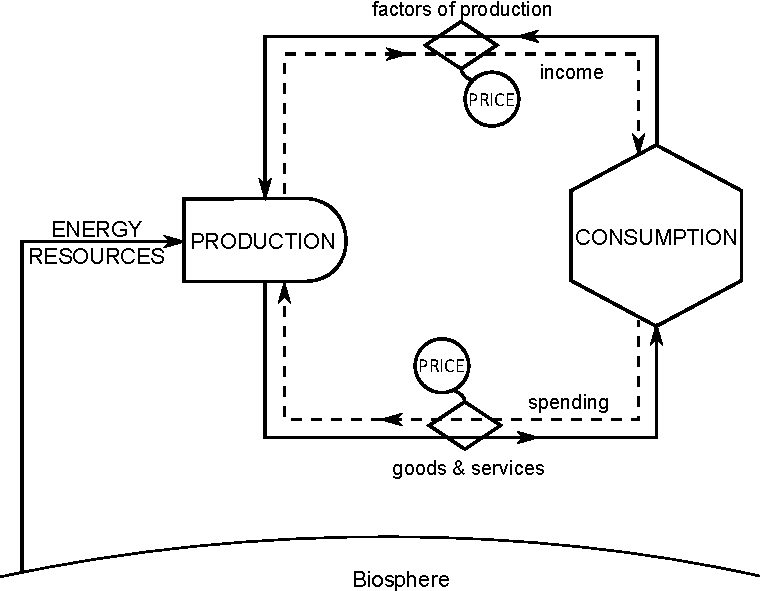
\includegraphics[width=\linewidth]{Part_0/Chapter_Introduction/images/Perpetual_motion_2.pdf}
\caption[The machine model]{The machine model of the economy includes
flows of energy into the economy from the biosphere.
This may be considered a perpetual motion machine 
of the second kind.}
\label{fig:perp_motion_2}
\end{figure}

The machine metaphor and engine model,
like the clockwork metaphor and traditional model,
are mechanistic.
Much like the engines of the Industrial Revolution,
the economic engine is assumed to be well-behaved and amenable to control.
Even today, machine metaphors abound in our economic discussions.
We continue to speak of ``fueling'' the ``economic engine'' 
lest it should ``stall.''~\cite{Liu2012}
Like a well-running engine, the economy is assumed 
to be resilient to small or even quite large perturbations.  
It can either self-correct, 
or be corrected predictably with adjustments to
a few policy levers.

But how accurate is the engine model?

According to the Second Law of Thermodynamics,
all real-world processes involve the degradation
of material and, especially, energy resources
and the creation of entropy.  
High quality (low entropy) material and energy come in;
low quality (high entropy) material and energy go out.
Wastes exist!
The depiction of the economy in Figure~\ref{fig:perp_motion_2} 
can be classified as a perpetual motion machine
of the \emph{second kind}:
it perfectly converts energy resources into 
work~(useful energy services) without generating
any entropy,
in violation of the Second Law of Thermodynamics.
Because the generation of high entropy~(low quality)
output is a \emph{necessary} feature of \emph{all} processes 
(including economic processes),
the generation of wastes is a \emph{normal} feature of
economic processes,
not an anomaly.

We need a different model.
We need a new metahpor.


%%%%%%%%%% Economy is society's metabolism %%%%%%%%%%
\section{The economy is society's metabolism}
\label{sec:economy_metabolism}
%%%%%%%%%%

In our opinion, an apt metaphor for the economy should account for the following facts 
about real economies. 
Economies:

\begin{enumerate}
	\item{\label{itm:intake}intake material and energy from the biosphere}
	\item{\label{itm:internal_exchange}exchange materials, energy, and information internally}
	\item{\label{itm:discharge}discharge material and energy wastes to the biosphere}
	\item{\label{itm:energetic_costs}are affected by energetic costs}
	\item{\label{itm:scarcity}are affected non-linearly by scarcity 
			in the face of low substitutibility}
	\item{\label{itm:non-linear}can change non-linearly or in discrete steps with the potential 
			for structural transformation}
	\item{\label{itm:embodies}accumulate embodied energy in material stocks, and}
	\item{\label{itm:robust}maintain organizational structure despite changes 
			in their environment.%
				\footnote{We note that 
				several areas of the literature speak to the items in this list.
				Material Flow Analysis~(MFA) and 
				Economy-Wide Material Flow Analys~(EW-MFA)
				stress the importance of
				material intake by the economy. 
				(See Section~\ref{sec:materials_auto}.)
				The Input-Output~(I-O) method highlights the effects of internal exchanges
				of material and information with economies. 
				(See Chapter~\ref{chap:intensity}.)
				Life-Cycle Assessment~(LCA) techniques focus attention 
				on otherwise-neglected wastes. 
				(See Section~\ref{sec:intensity_auto}.)
				Net Energy Analysis~(NEA) predicts that energy resource 
				scarcity reduces Energy Return on Investment~(EROI)
				and increases energy prices.
				(See Sections~\ref{sec:B_energy} 
				and~\ref{sec:resource_quality_and_irreversibility}.)
				The Energy Input-Output~(EI-O) method gives prominence to energetic costs
				of internal material and energy flows.
				(See Chapter~\ref{chap:intensity}.)
				And, thermodynamic control-volume modeling describes
				transient behavior and system transformations.
				(See Chapters~\ref{chap:materials}--\ref{chap:value}.)
			}}
\end{enumerate}

Living metabolisms%
	\footnote{The 
	Greek root of metabolism 
	(\emph{metabol$\bar{e}$}) means ``change.''}
exhibit the characteristics in the list above.
Metabolisms and the organisms they support
are intimately connected with the biosphere:
they withdraw materials and energy from the biosphere~(\ref{itm:intake}), 
transfer materials and energy internally via metabolic processes~(\ref{itm:internal_exchange}),
and discharge wastes back to the biosphere~(\ref{itm:discharge});
in fact, their very survival depends on these processes.
Extending Figures~\ref{fig:perp_motion_1} and~\ref{fig:perp_motion_2}
to include the facts in items~(\ref{itm:intake})--(\ref{itm:discharge}), % chktex 36
we obtain Figure~\ref{fig:metabolic_economy}.
Metabolisms are affected by energetic costs~(\ref{itm:energetic_costs}): 
an organism that obtains less energy than it expends is doomed.
Withholding life-sustaining resources brings drastic, non-linear
consequences for any metabolism~(\ref{itm:scarcity}).
Metabolisms enable non-linear, structural transformations
in their host organisms (e.g., metamorphosis, puberty, and evolution)~(\ref{itm:non-linear}).
And, energy absorbed by a metabolism is considered to be ``embodied''
in the cells of the organism~(\ref{itm:embodies}).
Metabolisms exist in a state of dynamic stability~(\ref{itm:robust}),
adjusting and readjusting to maintain their internal conditions
despite changes in the environment;
for a metabolism, equilibrium means death!

The economy is society's metabolism.\cite{Giampietro2000, Giampietro2013, F-K1999}

\begin{figure}[!ht]
\centering\
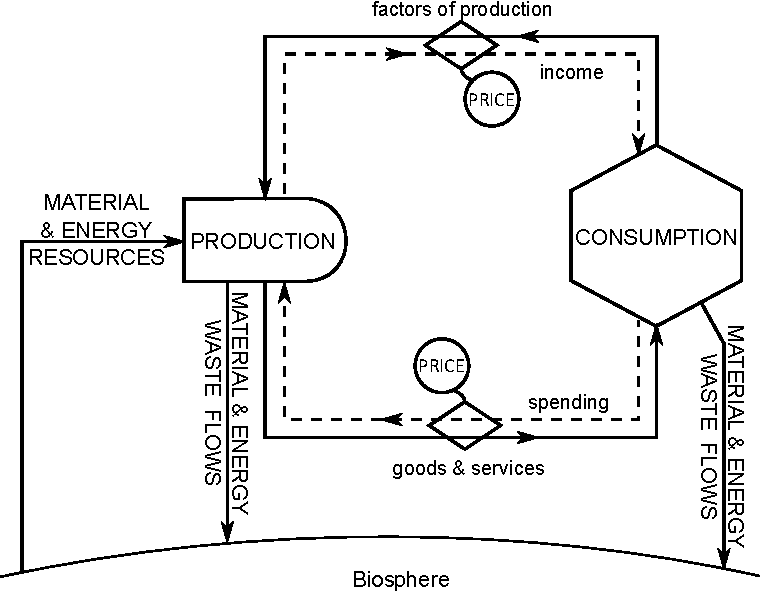
\includegraphics[width=\linewidth]{Part_0/Chapter_Introduction/images/PERKS.pdf}
\caption[The metabolism model]{The metabolism model provides a comprehensive view 
of the economy, fully consistent with the laws of thermodynamics, 
including degraded resources (waste) expelled 
to the environment as a necessary consequence of economic activity.}
\label{fig:metabolic_economy}
\end{figure}

Although we're not the first to utilize the metabolism metaphor,
[Fischer-Kowalski; Gowdy; Heijman; Liu; Giamietro]
we believe that, to date, 
the metabolism metaphor has not been utilized to the full extent possible. 
In practical terms, the metabolism metaphor is under-utilized
because national accounting continues to operate
under the assumptions of the machine metaphor and engine model
(Section~\ref{sec:machine_metaphor}).%
	 \footnote{As discussed above, the purpose of this book is to 
	 provide a rigorous theoretical framework for comprehensive national accounting.
	 To that end, we'll utilize the metabolic metaphor 
	 in the chapters that follow.
	 }
**** Verify with Becky that this is still the case. **** 
In theoretical terms, the metabolism metaphor is under-utilized because 
most researchers (with the exception of Giampietro~\cite{Giampietro2000, Giampietro2013})
use the metabolism metaphor to frame analyses of
(a) material flows into, through, and out of the economy for the purpose of understanding 
(b) stocks of raw materials in the biosphere.%
	\footnote{The field most closely associated with the metabolism metaphor is
	Materials Flow Analysis (MFA). 
	To be fair, materials flow analysts clearly acknowledge that 
	materials flow into the economy (minerals and ores, especially),
	in part,
	for the purpose of building up stocks of technical infrastructure (buildings),
	livestock, and people.\cite[p.~116]{F-K1999} 
	However, there is little emphasis on quantifying \emph{levels} 
	of material stock in Materials \emph{Flow} Analysis, 
	as its name implies.
	In fact, the equations in MFA~\cite[Equation~1]{F-K1999} are almost always written as%
	\[
		inflow = outflow + accumulation,
	\]
	reflecting the focus on flows.
	In this book, similar equations 
	(see Equation~\ref{eq:general_accumulation_equation}) 
	are written as%
	\[
		accumulation = inflow - outflow,
	\]
	thereby focusing on accumulation.
	}
If effect, this is the same oversight as national accounting: 
under-appreciation of the important role of societal material stocks 
in determining material and energy demand 
for the emplacement, use, maintenance, and replacement of the very same stocks.

It becomes a vicious cycle. 
By not including these factors in national accounting, 
society is blind to the important role that societal material stocks play.
Because society under-appreciates the role of material stocks in the economy, 
there is little urgency to include those stocks in national accounting.

We think that a deeper understanding of the metabolic metaphor
can both highlight the importance of societal material stocks and 
provide the basis for a rigorous theoretical framework 
for comprehensive national accounting.
In the following sections, 
we extend the metabolism metaphor in ways that are helpful 
for deepening our understanding the role of societal material stocks
and for building a rigorous theoretical framework 
for comprehensive national accounting.


%+++++++++ Anabolism ++++++++++
\subsection{Anabolism}
\label{sec:anabolism}
%+++++++++

Metabolic processes are classified as anabolic and catabolic 
(Section~\ref{sec:catabolism}).

Anabolic process build up material stocks with the body (bones, muscle mass, tissues).

As it happens, larger organisms (with more accumulated stock)
require larger material flow rates compared to smaller bodies, even at rest.


%+++++++++ Catabolism ++++++++++
\subsection{Catabolism}
\label{sec:catabolism}
%+++++++++

Catabolic processes break down and destroy material stocks within an organism
through an oxidation process.
At the cellular level, catabolic oxidation releases chemical free energy, 
some of which synthesizes ATP, 
thereby providing energy to cells. 
The rest of the released energy is manifest as waste heat.
One of the waste products of cellular catabolim is CO$_2$.

The analogy between catabolic processes and the work 
of the energy sector in the economy is striking.
Power plants (fired by coal, oil, and natural gas) break down fossil fuels
in an oxidation process (combustion) to produce useful energy 
(typically, electricity or mechanical drive), 
thereby providing energy to other sectors of the economy.
Both waste heat and CO$_2$ are byproducts of combustion.

One catabolic pathway, autophagy, 
involves the breakdown of damaged, unneeded, or dysfunctional cellular compoenents 
(protiens and cell organelles)
for the purpose of re-use within the organism. 
Autophagy can be an adaptive response to low calorie intake,
promoting cell survival.

Again, the analogy between cellular metabolism and the economy is striking.
Whereas cellular autophagy repurposes proteins and cell organelles
for re-use by an organism,
recycling repurposes degraded
yet economically-valuable materials
for re-use by the economy.
Furthermore, recycling can also be an adaptive response 
to reduced material and energy inputs.
One famous example of this can be found on the streets of Cuba.
In the face of economic sanctions,
government restrictions on vehicle purchases, and
high import tariffs,
automobile imports by Cuba are very low.
As a result, Cuba hyper-recycles autos that were imported
prior to sanctions and manufactures replacement parts locally.
The average lifespan of automobiles has been extended
such that an estimated 60,000, pre-1960 cars~\cite{Schweid:2004aa} 
(so-called ``yank tanks'') are in service on the island.%
	\footnote{Despite the recent change allowing new car purchases by individuals,
	astronomical import taxes mean that Cuban streets remain populated 
	with vintage 1950s autos.\cite{Ramey:2014aa}
	}
(See Figure~\ref{fig:vintage_autos_cuba}.)

\begin{figure}[!ht]
\centering\
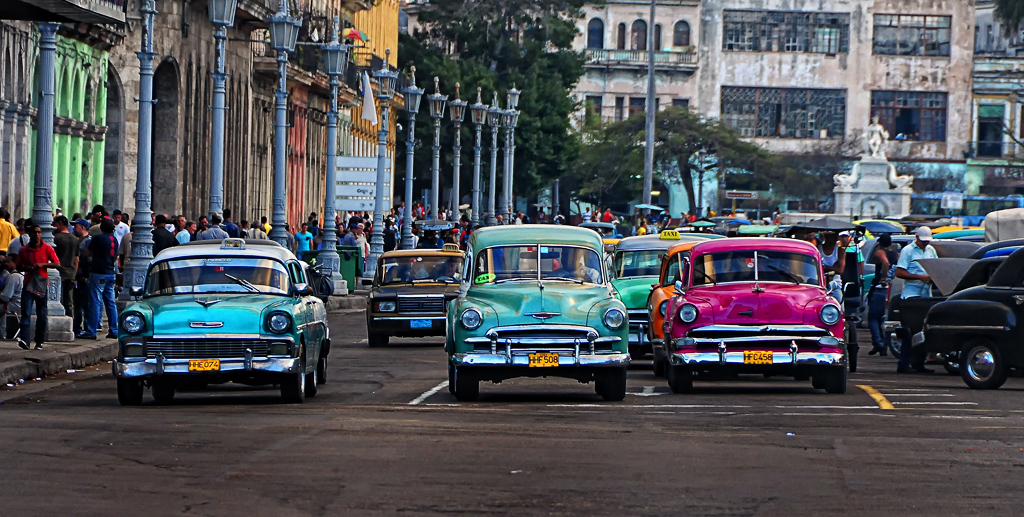
\includegraphics[width=4.5 in]{Part_0/Chapter_Acct_For_WoN/images/old-cars-of-cuba-dsc_4474-1024.jpg}
\caption[Vintage cars in Cuba]{Vintage cars (``yank tanks'') in Cuba.
**** This image is from 
\url{http://lcowlesphotography.wordpress.com/2011/02/13/old-cars-of-cuba/}.
What must we do to obtain the rights to the image? ****}
\label{fig:vintage_autos_cuba}
\end{figure}

If we can't obtain rights to Figure~\ref{fig:vintage_autos_cuba}, 
other options include:

\url{http://myadventuresacrosstheworld.wordpress.com/2013/03/14/transportation-in-cuba-old-cars-historical-cars-cocotaxi-bicitaxi-camionetas-and-what-not/}

\url{http://www.travelforboomers.com/2012/10/17/so-close-and-yet-so-far-away-viva-cuba/}

\url{http://ocean.otr.usm.edu/~w301497/travels/cuba2010/cuba2010b.html}



%+++++++++ Scale ++++++++++
\subsection{Issues of scale}
\label{sec:metabolic_scale}
%+++++++++

All organisms (and their metabolisms) 
exist within the context of the encompassing biosphere.
A booming population that consumes its food supply (energy) 
at a rate higher than it can be replenished
will experience a die-off (bust).
In nature, it is clear that the physical size (``scale'') of an organism 
(and the population of its species) realtive to the biosphere
is a determinitive factor for survival.
Such dynamics of boom-bust cycles of species population are
well-known to systems ecologists.

The economic analogy is a ``Malthusian'' economy.
When an economy grows to the point where it is consuming food 
at a faster rate than it is grown,
population declines in what is known as a ``Malthusian catastrophe.''
**** Becky, can you fill in some details here and in the following paragraph? ****

Interestingly, no systems ecologist would contend that 
a species is free from the boom-bust cycles caused by biosphere constraints.
However, economists claim that many economies have escaped the ``Malthusian trap''
in that (to date) the incredible population boom
of the industrial revolution has not been followed by a population bust.

\begin{figure}[!ht]
\centering\
\includegraphics[width=4.5 in]{Part_0/Chapter_Acct_For_WoN/images/population.jpg}
\caption[World population]{World population.
**** This image is from 
\url{http://www.truthmove.org/workspace/photos-content/WorldPopulationGraph_yearPre7000BCto2025AD_metalAges_703x578.jpg}.
Becky: can you obtain the data and put it in Excel? ****}
\label{fig:population}
\end{figure}









Hypermetabolism (http://en.wikipedia.org/wiki/Hypermetabolism).








%%%%%%%%%% Metabolism metaphor helps %%%%%%%%%%
\section{[MKH] Metabolism metaphor assists understanding}
\label{sec:metabolism_helps}
%%%%%%%%%%

In Chapter~\ref{chap:acct_for_won}.



%%%%%%%%%% What would change %%%%%%%%%%
\section{[BRH] What would change}
\label{sec:what_would_change}
%%%%%%%%%%

In Chapter~\ref{chap:acct_for_won}.



%%%%%%%%%% Rigorous framework %%%%%%%%%%
\section{[MKH] Rigorous framework}
\label{sec:rigorous_framework}
%%%%%%%%%%

In Chapter~\ref{chap:acct_for_won}.


Here are are some citations in Chapter 2.~\cite{Berry:1973vo}


\bibliographystyle{unsrt}
\bibliography{../../Metabolic}


% Always give a unique label
% and use \ref{<label>} for cross-references
% and \cite{<label>} for bibliographic references
% use \sectionmark{}
% to alter or adjust the section heading in the running head
%% Instead of simply listing headings of different levels we recommend to let every heading be followed by at least a short passage of text. Furtheron please use the \LaTeX\ automatism for all your cross-references and citations.

%% Please note that the first line of text that follows a heading is not indented, whereas the first lines of all sequent paragraphs are.

%% Use the standard \verb|equation| environment to typeset your equations, e.g.
%
%% \begin{equation}
%% a \times b = c\;,
%% \end{equation}
%
%% however, for multiline equations we recommend to use the \verb|eqnarray|
%% environment\footnote{In physics texts please activate the class option \texttt{vecphys} to depict your vectors in \textbf{\itshape boldface-italic} type - as is customary for a wide range of physical jects.}.
%% \begin{eqnarray}
%% a \times b = c \nonumber\\
%% \vec{a} \cdot \vec{b}=\vec{c}
%% \label{eq:01}
%% \end{eqnarray}

%% \section{section Heading}
%% \label{sec:2}
%% Instead of simply listing headings of different levels we recommend to let every heading be followed by at least a short passage of text. Furtheron please use the \LaTeX\ automatism for all your cross-references\index{cross-references} and citations\index{citations} as has already been described in Sect.~\ref{sec:2}.

%% \begin{quotation}
%% Please do not use quotation marks when quoting texts! Simply use the \verb|quotation| environment -- it will automatically render Springer's preferred layout.
%% \end{quotation}


%% \section{section Heading}
%% Instead of simply listing headings of different levels we recommend to let every heading be followed by at least a short passage of text. Furtheron please use the \LaTeX\ automatism for all your cross-references and citations as has already been described in Sect.~\ref{sec:2}, see also Fig.~\ref{fig:1}\footnote{If you copy text passages, figures, or tables from other works, you must obtain \textit{permission} from the copyright holder (usually the original publisher). Please enclose the signed permission with the manucript. The sources\index{permission to print} must be acknowledged either in the captions, as footnotes or in a separate section of the book.}

%% Please note that the first line of text that follows a heading is not indented, whereas the first lines of all sequent paragraphs are.

% For figures use
%
%% \begin{figure}[b]
%% \sidecaption
% Use the relevant command for your figure-insertion program
% to insert the figure file.
% For example, with the option graphics use
%% \includegraphics[scale=.65]{figure}
%
% If not, use
%\picplace{5cm}{2cm} % Give the correct figure height and width in cm
%
%% \caption{If the width of the figure is less than 7.8 cm use the \texttt{sidecapion} command to flush the caption on the left side of the page. If the figure is positioned at the top of the page, align the sidecaption with the top of the figure -- to achieve this you simply need to use the optional argument \texttt{[t]} with the \texttt{sidecaption} command}
%% \label{fig:1}       % Give a unique label
%% \end{figure}


%% \paragraph{Paragraph Heading} %
%% Instead of simply listing headings of different levels we recommend to let every heading be followed by at least a short passage of text. Furtheron please use the \LaTeX\ automatism for all your cross-references and citations as has already been described in Sect.~\ref{sec:2}.

%% Please note that the first line of text that follows a heading is not indented, whereas the first lines of all sequent paragraphs are.

%% For typesetting numbered lists we recommend to use the \verb|enumerate| environment -- it will automatically render Springer's preferred layout.

%% \begin{enumerate}
%% \item{Livelihood and survival mobility are oftentimes coutcomes of uneven socioeconomic development.}
%% \begin{enumerate}
%% \item{Livelihood and survival mobility are oftentimes coutcomes of uneven socioeconomic development.}
%% \item{Livelihood and survival mobility are oftentimes coutcomes of uneven socioeconomic development.}
%% \end{enumerate}
%% \item{Livelihood and survival mobility are oftentimes coutcomes of uneven socioeconomic development.}
%% \end{enumerate}


%% \paragraph{paragraph Heading} In order to avoid simply listing headings of different levels we recommend to let every heading be followed by at least a short passage of text. Use the \LaTeX\ automatism for all your cross-references and citations as has already been described in Sect.~\ref{sec:2}, see also Fig.~\ref{fig:2}.

%% Please note that the first line of text that follows a heading is not indented, whereas the first lines of all sequent paragraphs are.

%% For unnumbered list we recommend to use the \verb|itemize| environment -- it will automatically render Springer's preferred layout.

%% \begin{itemize}
%% \item{Livelihood and survival mobility are oftentimes coutcomes of uneven socioeconomic development, cf. Table~\ref{tab:1}.}
%% \begin{itemize}
%% \item{Livelihood and survival mobility are oftentimes coutcomes of uneven socioeconomic development.}
%% \item{Livelihood and survival mobility are oftentimes coutcomes of uneven socioeconomic development.}
%% \end{itemize}
%% \item{Livelihood and survival mobility are oftentimes coutcomes of uneven socioeconomic development.}
%% \end{itemize}

%% \begin{figure}[t]
%% \sidecaption[t]
% Use the relevant command for your figure-insertion program
% to insert the figure file.
% For example, with the option graphics use
%% \includegraphics[scale=.65]{figure}
%
% If not, use
%\picplace{5cm}{2cm} % Give the correct figure height and width in cm
%
%% \caption{Please write your figure caption here}
%% \label{fig:2}       % Give a unique label
%% \end{figure}

%% \runinhead{Run-in Heading Boldface Version} Use the \LaTeX\ automatism for all your cross-references and citations as has already been described in Sect.~\ref{sec:2}.

%% \runinhead{Run-in Heading Italic Version} Use the \LaTeX\ automatism for all your cross-refer\-ences and citations as has already been described in Sect.~\ref{sec:2}\index{paragraph}.
% Use the \index{} command to code your index words
%
% For tables use
%
%% \begin{table}
%% \caption{Please write your table caption here}
%% \label{tab:1}       % Give a unique label
%
% For LaTeX tables use
%
%% \begin{tabular}{p{2cm}p{2.4cm}p{2cm}p{4.9cm}}
%% \hline\noalign{\smallskip}
%% Classes & class & Length & Action Mechanism  \\
%% \noalign{\smallskip}\svhline\noalign{\smallskip}
%% Translation & mRNA$^a$  & 22 (19--25) & Translation repression, mRNA cleavage\\
%% Translation & mRNA cleavage & 21 & mRNA cleavage\\
%% Translation & mRNA  & 21--22 & mRNA cleavage\\
%%Translation & mRNA  & 24--26 & Histone and DNA Modification\\
%%\noalign{\smallskip}\hline\noalign{\smallskip}
%%\end{tabular}
%%$^a$ Table foot note (with superscript)
%%\end{table}
%
%% \section{Section Heading}
%%\label{sec:3}
% Always give a unique label
% and use \ref{<label>} for cross-references
% and \cite{<label>} for bibliographic references
% use \sectionmark{}
% to alter or adjust the section heading in the running head
%% Instead of simply listing headings of different levels we recommend to let every heading be followed by at least a short passage of text. Furtheron please use the \LaTeX\ automatism for all your cross-references and citations as has already been described in Sect.~\ref{sec:2}.

%% Please note that the first line of text that follows a heading is not indented, whereas the first lines of all sequent paragraphs are.

%%If you want to list definitions or the like we recommend to use the Springer-enhanced \verb|description| environment -- it will automatically render Springer's preferred layout.

%%\begin{description}[Type 1]
%%\item[Type 1]{That addresses central themes pertainng to migration, health, and disease. In Sect.~\ref{sec:1}, Wilson discusses the role of human migration in infectious disease distributions and patterns.}
%%\item[Type 2]{That addresses central themes pertainng to migration, health, and disease. In Sect.~\ref{sec:2}, Wilson discusses the role of human migration in infectious disease distributions and patterns.}
%%\end{description}

%%\section{section Heading} %
%% In order to avoid simply listing headings of different levels we recommend to let every heading be followed by at least a short passage of text. Use the \LaTeX\ automatism for all your cross-references and citations citations as has already been described in Sect.~\ref{sec:2}.

%% Please note that the first line of text that follows a heading is not indented, whereas the first lines of all sequent paragraphs are.

%% \begin{svgraybox}
%% If you want to emphasize complete paragraphs of texts we recommend to use the newly defined Springer class option \verb|graybox| and the newly defined environment \verb|svgraybox|. This will produce a 15 percent screened box 'behind' your text.

%% If you want to emphasize complete paragraphs of texts we recommend to use the newly defined Springer class option and environment \verb|svgraybox|. This will produce a 15 percent screened box 'behind' your text.
%% \end{svgraybox}


%% \section{section Heading}
%%Instead of simply listing headings of different levels we recommend to let every heading be followed by at least a short passage of text. Furtheron please use the \LaTeX\ automatism for all your cross-references and citations as has already been described in Sect.~\ref{sec:2}.

%% Please note that the first line of text that follows a heading is not indented, whereas the first lines of all sequent paragraphs are.

%% \begin{theorem}
%% Theorem text goes here.
%% \end{theorem}
%
% or
%
%% \begin{definition}
%% Definition text goes here.
%% \end{definition}

%% \begin{proof}
%\smartqed
%% Proof text goes here.
%% \qed
%% \end{proof}

%%\paragraph{Paragraph Heading} %
%% Instead of simply listing headings of different levels we recommend to let every heading be followed by at least a short passage of text. Furtheron please use the \LaTeX\ automatism for all your cross-references and citations as has already been described in Sect.~\ref{sec:2}.

%% Note that the first line of text that follows a heading is not indented, whereas the first lines of all subsequent paragraphs are.
%
% For built-in environments use
%
%%\begin{theorem}
%%Theorem text goes here.
%%\end{theorem}
%
%%\begin{definition}
%%Definition text goes here.
%%\end{definition}
%
%%\begin{proof}
%%\smartqed
%% Proof text goes here.
%%\qed
%%\end{proof}
%
%% \begin{acknowledgement}
%% If you want to include acknowledgments of assistance and the like at the end of an individual chapter please use the \verb|acknowledgement| environment -- it will automatically render Springer's preferred layout.
%% \end{acknowledgement}
%
%% \section*{Appendix}
%% \addcontentsline{toc}{section}{Appendix}
%
%% When placed at the end of a chapter or contribution (as opposed to at the end of the book), the numbering of tables, figures, and equations in the appendix section continues on from that in the main text. Hence please \textit{do not} use the \verb|appendix| command when writing an appendix at the end of your chapter or contribution. If there is only one the appendix is designated ``Appendix'', or ``Appendix 1'', or ``Appendix 2'', etc. if there is more than one.

%% \begin{equation}
%% a \times b = c
%% \end{equation}
% Problems or Exercises should be sorted chapterwise
%% \section*{Problems}
%% \addcontentsline{toc}{section}{Problems}
%
% Use the following environment.
% Don't forget to label each problem;
% the label is needed for the solutions' environment
%% \begin{prob}
%% \label{prob1}
%% A given problem or Excercise is described here. The
%% problem is described here. The problem is described here.
%% \end{prob}

%% \begin{prob}
%% \label{prob2}
%% \textbf{Problem Heading}\\
%% (a) The first part of the problem is described here.\\
%% (b) The second part of the problem is described here.
%% \end{prob}


